\section{Demonstration Setup}
\label{sec:demo}

The heart of our demo is a live web interface which is 
implemented in PHP on top of the
partial suppression system \footnote{The demo can be accessed at
\url{http://adapt.seiee.sjtu.edu.cn/SetDemo}.}. The web interface and
partial suppression prototype system are both deployed on the same 
server machine which sports 4 Intel processors and 39GB of RAM. 
Our demo consists of two main sessions:
LiveDemo and Benchmark.

In the LiveDemo session, we offer two options in which a user can either try
to experience the partial suppression system with supplied benchmark or
create her own data to anonymize. A screen-shot of the LiveDemo section is
shown in Figure \ref{fig:gui}. By selecting one of the supplied dataset,
varying the confidence threshold which defines acceptable upper-bounded
confidence for safe sensitive association rules and clicking the submit
button, you will start the live experiment. On the other side, user
customizable input is also permitted with minor constraints in input format
and input size. During the process, the input dataset is first parsed and
verified by the web interface, and then it is transformed to the required
format and handed over to the background partial suppression system 
for processing. Subsequently the result is displayed on the
web interface. Our demo system provides the suppression summary
and the detailed suppressed data as the partial suppression output.
%is shown in Figure \ref{fig:demooutput},
%as you can see, we
%demonstrate both the suppression summary and the detailed suppressed data.

\begin{figure}[th]
	\centering
	\epsfig{file=pic/livedemo.eps,width=\columnwidth}
\caption{Web Demo GUI: LiveDemo}
\label{fig:gui}
\end{figure}

In Benchmark session, we list all the experimental datasets mentioned in this
paper. By clicking on the any one of them, you will both see the detailed
description of the data and the data itself, which helps you to better know
how the data looks like.
%, these are both shown in Figure
%\ref{fig:benchmark}.

%\begin{figure}[th]
%	\centering
%	\epsfig{file=benchmark.eps,width=0.9\columnwidth}
%\caption{Web Demo GUI: Benchmark}
%\label{fig:benchmark}
%\end{figure}

Due to bandwidth and system load constraint of the web server,
we allow only one partial suppressor running at a time. Therefore, only one
user can access the demo at this time.
